\subsection{Arbitrary Convex n-gons}
% polish: check that no orientation (left, right, ...) and cw/ccw is used undefined

In this section we give a detailed overview of \cite{shitov2020sublinear}, which proves $\xc(P) \in O(n^{2/3})$ for any $n$-gon $P$.
We focus on the underlying ideas and present only important arguments in more detail. In contrast to the source, we start the proof ``backwards'', presenting  the results first, since in doing so, we can highlight the reasoning more clearly.

The gist of the approach is as follows:
\begin{enumerate}
  \item We cut the polygon into smaller slices, for which we can provide small extended formulations. Joining these together preserves this property.
  \item We prove this small extended formulation by iteratively finding a large enough subset of vertices in the slice, for which we can build a small extended formulation. Joining these subsets together will again preserve this property.
  \item We build the small extended formulation by building 3-dimensional extended formulations for a surrounding polygon. These are ``glued'' together resulting in an extended formulation for the original set of vertices.
\end{enumerate}

In Appendix~\ref{sec:dependency-graph} we added a graphical representation of the dependencies in the proofs of \cite{shitov2014sublinear}. It may be of help in understanding how the statements lead to the main result or how some statements are connected.



\subsubsection{Main Result}

\begin{theorem}[{\cite[Theorem 5]{shitov2020sublinear}}]\label{theorem:xc}
  Every convex $n$-gon $P$ has $\xc(P) \leq 147 n^{2/3}$.
\end{theorem}

Naturally, we need to gather more statements, before we can prove this theorem.

The starting point is the following lemma, adopted from \cite[Proposition 3.1.1]{weltge2015sizes}, which states that the extension complexity behaves well for unions of polytopes:
\begin{lemma}[{\cite[Lemma 8]{shitov2020sublinear}}]\label{lemma:union}
  Let $P$ and $Q$ be polytopes in $\R^d$ -- each different from a point\footnote{In regards to polygons, one is tempted to think of these polytopes as being disjunct. But they can be arranged arbitrarily.}. Then $$\xc(\conv(P \cup Q)) \leq \xc(P) + \xc(Q) .$$
\end{lemma}

This lemma allows us to consider a polygon in parts, when estimating its extension complexity, since we can bound the total complexity by the sum of its parts.

Now we will go on to define those smaller parts, which we can handle well.

\begin{definition}[Turning angle]
  If $P\subset\R^2$ is a polygon, then the \emph{turning angle} at a vertex $v$ is $\pi-\angle v_-vv_+$, where $v_-$ and $v_+$ are two vertices adjacent to $v$ in $P$. \\
  In other words, it is the amount the angle at $v$ deviates from a straight line. \\
  The \emph{turning angle} of an edge $e$ of a polygon is the sum of the turning angles at the two endpoints of $e$.
\end{definition}

\begin{definition}[Correct sequence]
  A sequence $v=(v_1,\ldots,v_n)$ of distinct points on a plane is called \emph{correct} if these points are the vertices of their convex hull $P$ and the segment between any pair of consecutive points in $v$ is an edge of $P$.
  If not stated otherwise, we assume the vertices of a correct sequence to be ordered \emph{clockwise}.
\end{definition}

\begin{definition}[Thin sequence]
  Let $\alpha\in(0,\pi)$ and $n \geq 3$. A correct sequence ${v=(v_1,\ldots,v_n)}$ is called \emph{$\alpha$-thin}, if the turning angle of the edge $\conv\{v_1, v_n\}$ in the polygon $\conv v$ is greater than $2\pi-\alpha$, that is, $$\angle v_n v_1 v_2+\angle v_1v_nv_{n-1}<\alpha.$$ We say that $v$ is \emph{thin}, if it is $\alpha$-thin for some $\alpha\in(0,\pi)$.
\end{definition}

\begin{figure}[ht]
  \centering
  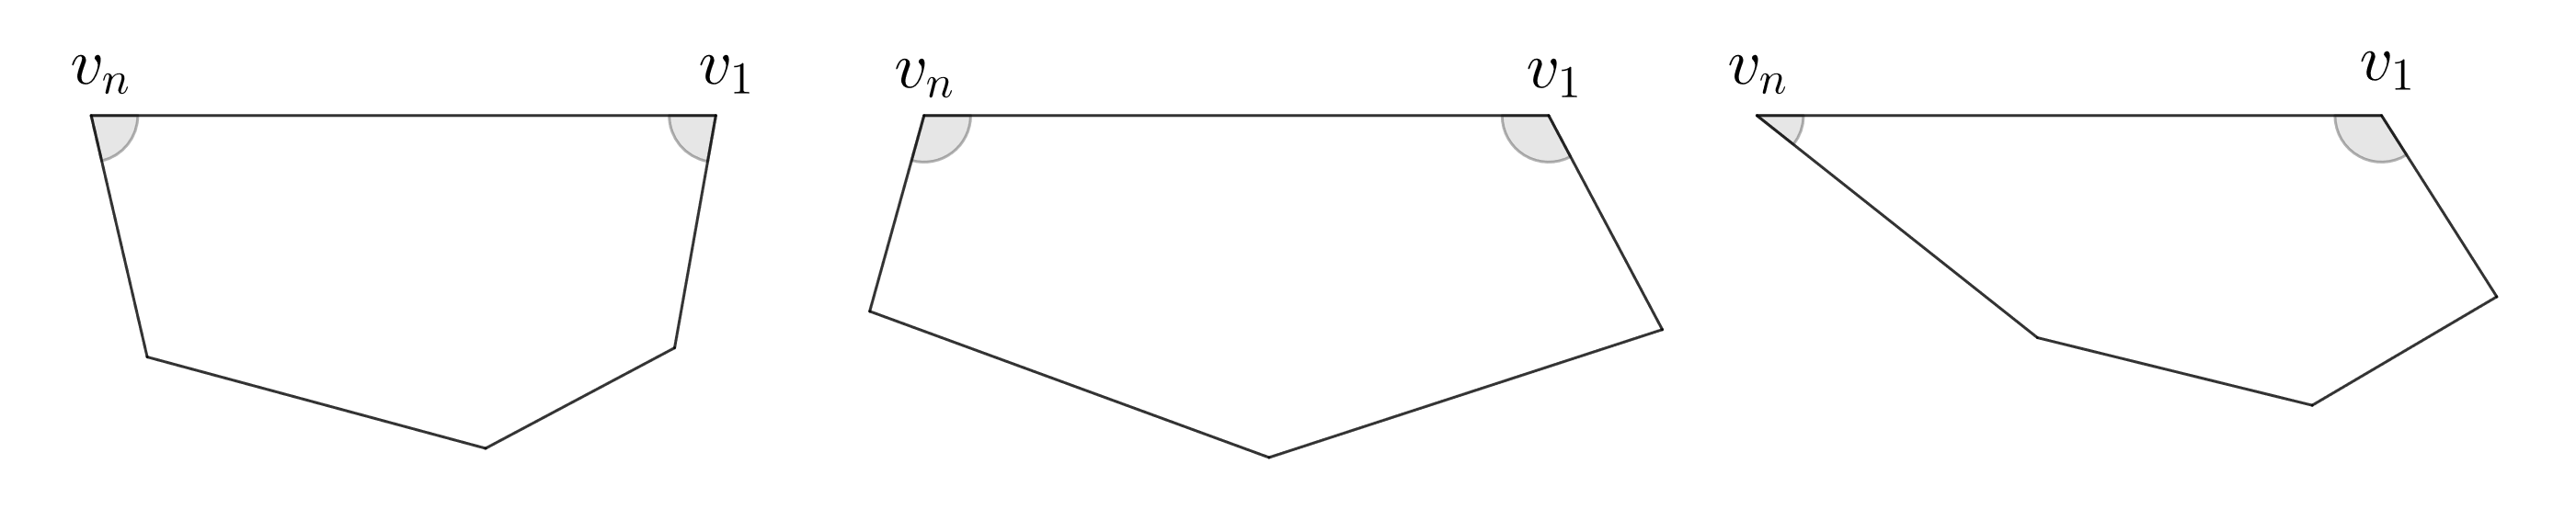
\includegraphics[width=\textwidth]{thin-seqeunce.png}
  \caption{Examples of thin and not-thin sequences: The sequence in the middle is the only one, which is \emph{not} thin.}
  \label{fig:thin-sequence}
\end{figure}

For thin sequences, all lines $v_i \wedge v_j$, where $\{i,j\} \neq \{1,n\}$, meet on the same side of $v_1 \wedge v_n$.

\begin{observation}[Splitting into thin sequences, {\cite[Observation 30]{shitov2020sublinear}}]\label{observation:splitting}
  Let $P$ be a convex polygon with $n$ vertices, and let $q \geq 3$ be an integer. Then the vertices of $P$ can be partitioned into at most $q$ sets each of which is either a point or a pair of points, or else a set that forms a $2\pi/q$-thin sequence.
\end{observation}

\begin{figure}[ht]
  \centering
  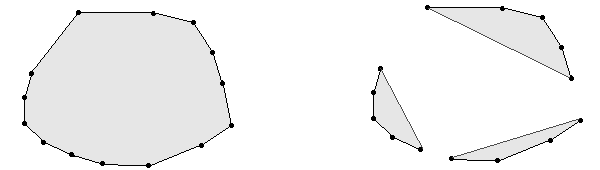
\includegraphics[width=80mm]{polygon-splitting.png}
  \caption{Splitting the vertices of a polygon into thin sequences. \cite[Figure 4]{shitov2020sublinear}}
  \label{fig:polygon-splitting}
\end{figure}

\begin{proof}[Proof outline]
  For each set, take as many vertices (in order) until the $2\pi/q$-thinness would be violated. Then begin a new set, which starts at least $2\pi/q$ further from the last -- so at most $q$ sets cover the polygon's vertices.
\end{proof}

Based on Observation~\ref{observation:splitting} we choose to split the original $n$-gon into $12$ distinct $\pi/6$-thin sequences. Joining those (constantly many) sequences will not change the asymptotical bound for the extension complexity of the original polygon in light of Lemma~\ref{lemma:union}.

Now we will go on to show that each $\pi/6$-thin sequence has extension complexity $O(n^{2/3})$. We do this by iteratively extracting a subsequence with a small extended formulation.

\begin{theorem}[{\cite[Theorem 58]{shitov2020sublinear}}]\label{theorem:subsequence}
  Let $v$ be a $\pi/6$-thin sequence with $n = 1024\tau^3 + 8\tau$ vertices, where $\tau \in \N$.
  Then $v$ contains a subsequence $u$ with $\abs{u} \geq 4\tau^2$ and $\xc(u) \leq 12\tau$.
\end{theorem}

Proving this theorem is the objective of the rest of the paper. We preempted it to provide a better understanding of the results.

The following corollary is a direct result of it:

\begin{corollary}[{\cite[Corollary 59]{shitov2020sublinear}}]\label{corollary:subsequence}
  Let $v$ be a $\pi/6$-thin sequence with $n > 263\,000$ vertices.
  Then $v$ contains a subsequence $u$ with $\abs{u} \geq \frac{1}{36}\,n^{2/3}$ and $\xc(s) \leq \left( \frac{72}{43}\,n \right)^{1/3}$.
\end{corollary}

\begin{proof}[Proof outline]
  Apply Theorem~\ref{theorem:subsequence} with $\tau=\left\lfloor (n/1032)^{1/3} \right\rfloor$, which gives the desired result for $n > 263\,000$.
\end{proof}

\begin{corollary}[{\cite[Corollary 60]{shitov2020sublinear}}]\label{corollary:thin-xc}
  Let $v$ be a $\pi/6$-thin sequence. Then $$\xc(v) \leq \frac{324}{\sqrt[3]{129}}\,n^{2/3} .$$
\end{corollary}

\begin{proof}[Proof outline]
  Use induction for $n > 263\,000$ ($n \leq 263\,000$ is trivial) and apply Corollary~\ref{corollary:subsequence} and Lemma~\ref{lemma:union} for the induction step: $$\xc(\conv v) \leq \frac{324}{\sqrt[3]{129}} \left(n-\frac{n^{2/3}}{36}\right)^{2/3}+\left(\frac{72n}{43}\right)^{1/3} < \frac{324}{\sqrt[3]{129}}\,n^{2/3}$$
\end{proof}

We can now prove the main result.

\begin{proof}[Proof outline of Theorem~\ref{theorem:xc}]
  Using Observation~\ref{observation:splitting} we split the $n$-gon $P$ into twelve disjoint $\pi/6$-thin sequences\footnote{Technically we have to consider the case, when a sequence has less than three points. We omit it, since it does not provide further insight.} with sizes $n_1,\dots,n_{12}$.

  We apply Lemma~\ref{lemma:union} and Corollary~\ref{corollary:thin-xc} and get $$\xc(P)\leq\frac{324}{\sqrt[3]{129}}\left(\sum\limits_{i=1}^{12}n_i^{2/3}\right)\leq\frac{324}{\sqrt[3]{129}}\left(12\left(\frac{n}{12}\right)^{2/3}\right) < 147\,n^{2/3} .$$
\end{proof}



\subsubsection{Building Small Extended Formulations}

Before we can determine the subsequences in Theorem~\ref{theorem:subsequence}, we need to find a way to build those extended formulations.

The key idea here is to omit some vertices to obtain a simpler surrounding polygon. For this polygon we build specific 3-dimensional extended formulations with respect to the omitted vertices. If we now ``glue'' those extended formulations together in a special way, we get an extended formulation for the original polygon with small extension complexity.

Before we can formulate this theorem, we have to introduce \emph{acute polyhedra} and \emph{acute diagrams}. These help us build the extensions for the surrounding polygon.

\begin{definition}[Acute Polyhedron]\label{definition:acute-polyhedron}
  Assume $P \subset \R^3$ is a polyhedron and $B$ is one of its facets. If all other facets $F \neq B$ of $P$
  share an edge with $B$ and
  the angle\footnote{The angle between two faces $A$ and $B$ with a common edge $e$ is defined as the angle between two oriented segments that lie on $A$ and $B$ respectively, have their origin on $e$ and are orthogonal to $e$.} between $B$ and $F$ is acute,
  then $P$ is called an \emph{acute polyhedron} with \emph{base} $B$.\footnote{Note that all facets lie on the same side of $B$. Since otherwise, $B$ would be no facet of $P$.}
\end{definition}

\begin{definition}[Main edge]
  An edge $e$ of an acute polyhedron with base $B$ is called \emph{main}, if exactly one endpoint of $e$ lies on $B$.
\end{definition}

\begin{figure}[ht]
  \centering
  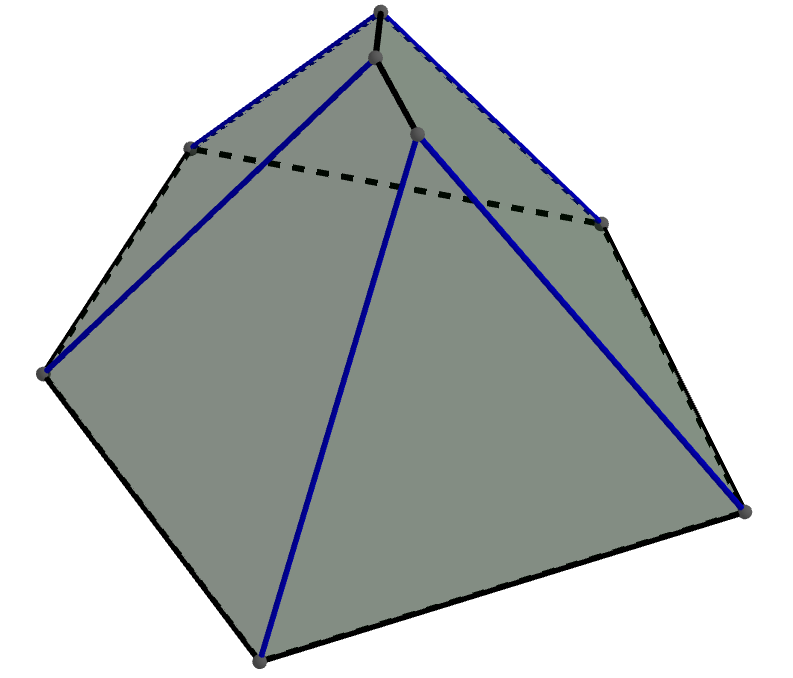
\includegraphics[width=70mm]{acute-polyhedron.png}
  \caption{An acute polyhedron with main edges colored.}
  \label{fig:acute-polyhedron}
\end{figure}

\begin{lemma}
  Any base vertex of an acute polyhedron belongs to a unique main edge.
\end{lemma}

\begin{proof}[Proof outline]
  A base vertex $v$ with two main edges would be contained in three non-base faces. Since they have to include $v$ and a base edge by Definition~\ref{definition:acute-polyhedron}, two of them coincide on the base, which is impossible for acute polyhedra.
\end{proof}

Now follows an important lemma, which allows us to construct an acute polyhedron for a given base, where all main edges but one have fixed direction with respect to the base.

\begin{lemma}[{\cite[Lemma 15]{shitov2020sublinear}}]\label{lemma:acute-direction}
  Let $V$ be a polygon with vertices $v_1,\dots,v_n$ and let $y_1,\dots,y_{n-1}$ be a set of inner points of $V$.
  Then there is an acute polyhedron $P$ with base $V$ such that, for any $i \in \{1,\dots,n-1\}$, the image of the main edge passing from $v_i$ under the orthogonal projection of $P$ onto $V$ is collinear to $v_i \wedge y_i$ \footnote{We use $x \wedge y$ to describe the line joining two points $x$ and $y$. It can also the intersection of two lines $x$ and $y$.}.
\end{lemma}

\begin{figure}[ht]
  \centering
  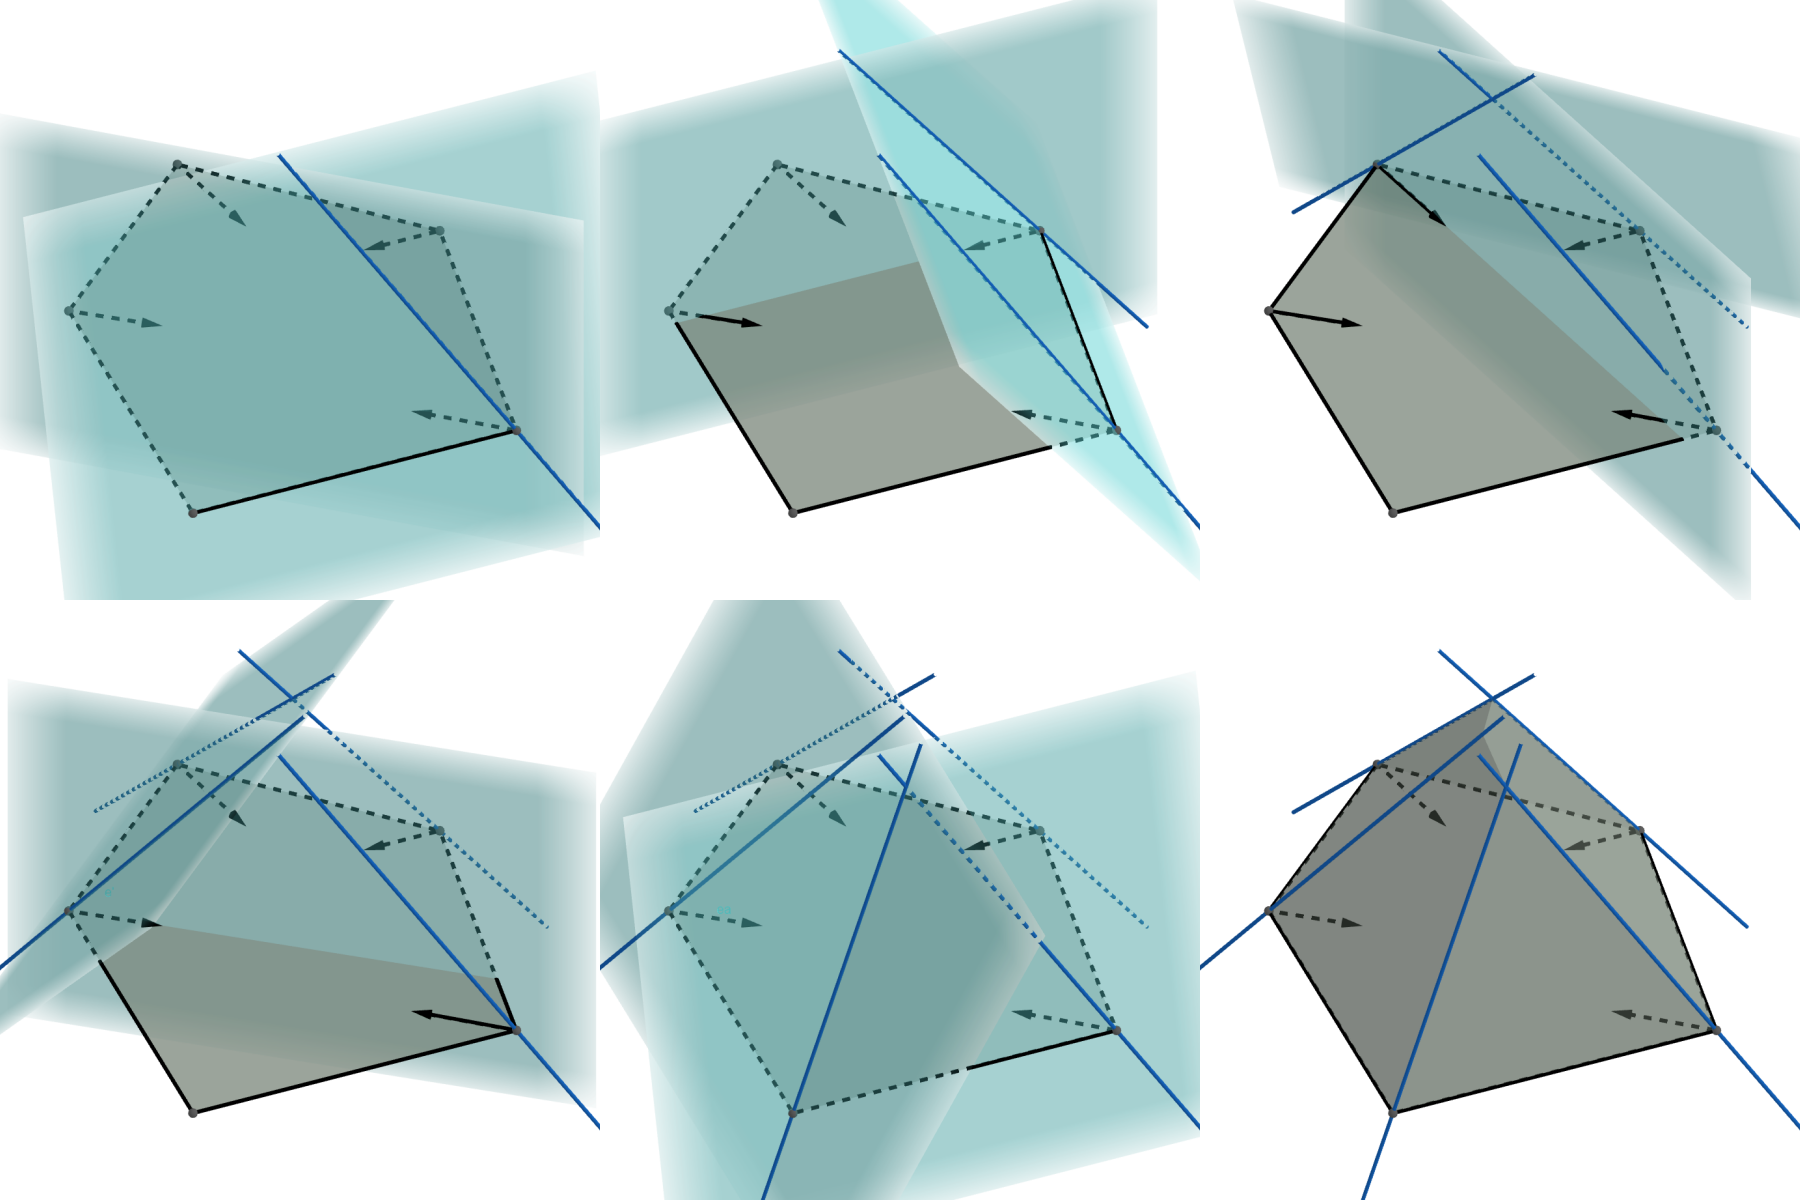
\includegraphics[width=\textwidth]{acute-construction.png}
  \caption{The construction of Figure~\ref{fig:acute-polyhedron} in the proof of Lemma~\ref{lemma:acute-direction}.}
  \label{fig:acute-construction}
\end{figure}

\begin{proof}[Proof outline (see Figure~\ref{fig:acute-construction})]
  Begin constructing a half-plane $F_n$ with base $v_n \wedge v_{n-1}$ and having an arbitrary acute angle with $V$. Define the plane $H_{n-1}$ orthogonal to $V$ containing $v_{n-1}$ and $y_{n-1}$. The half-plane $F_{n-1}$ has $v_{n-1} \wedge v_{n-2}$ as its base and contains $F_n \cap H_{n-1}$. Proceed this way until $F_1$ is constructed.\footnote{All $F_i$ have an acute angle with $V$, since they contain $F_{i+1} \cap H_i$, which is a ray with acute angle with~$V$.}
\end{proof}

\begin{observation}[{\cite[Observation 16]{shitov2020sublinear}}]\label{observation:acute-projection}
  Let $P$ be an acute polyhedron with base $B$.
  The orthogonal projection $\pi$ of $P$ onto the plane containing $B$ maps the non-base points of an acute polyhedron injectively into interior of $B$.
\end{observation}

\begin{proof}[Proof outline]
  Follows by definition of acute polyhedra (acute angle) and convexity of~$P$.
\end{proof}

\begin{definition}[Acute diagram and lifting]
  Let $P$ be an acute polyhedron with base~$B$ and $\pi$ like in Observation~\ref{observation:acute-projection}.
  The image of all edges of $P$ under $\pi$ gives us a diagram, which we call the \emph{acute diagram} of $P$ relative to base $B$.
  We also say that $P$ is an \emph{acute lifting} of the corresponding diagram.
\end{definition}

% polish: get image closer...
\begin{figure}[ht]
  \centering
  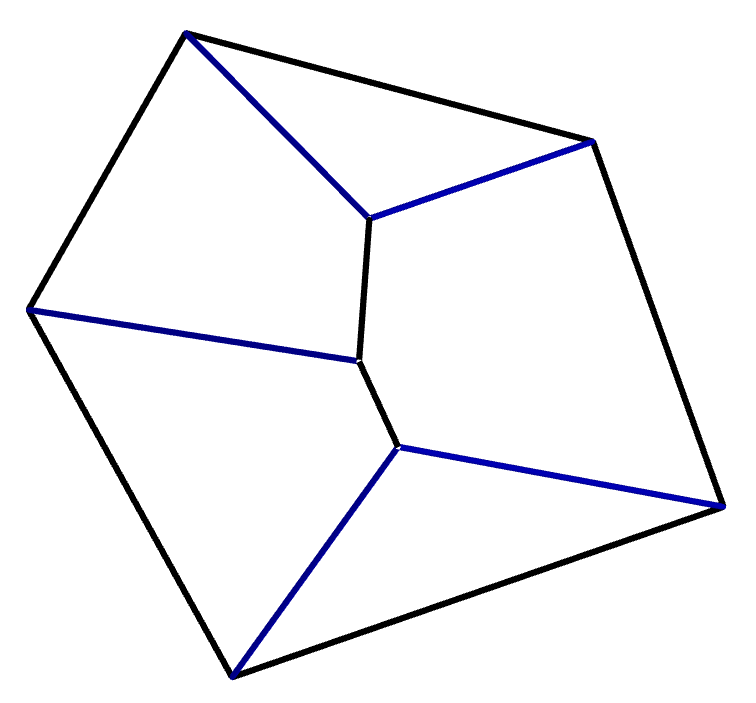
\includegraphics[width=70mm]{acute-diagram.png}
  \hspace*{5mm}
  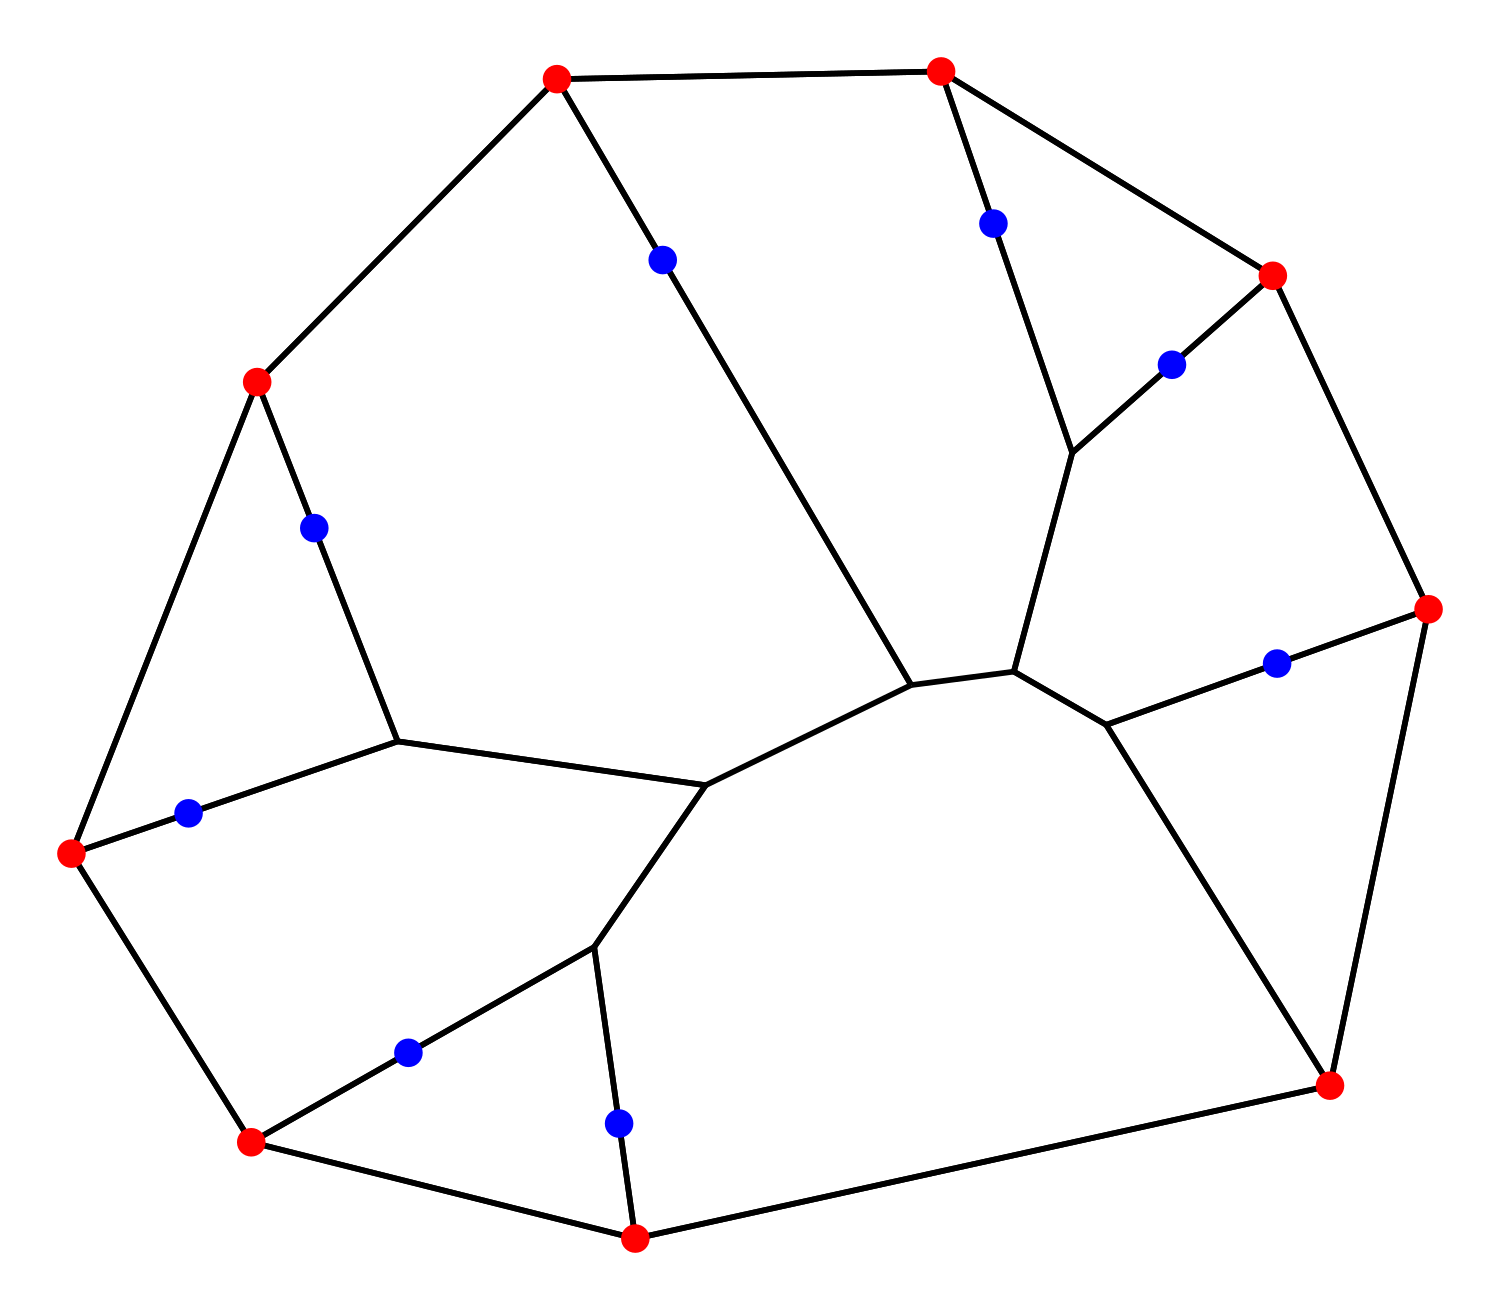
\includegraphics[width=70mm]{acute-diagram-2.png}
  \caption{The acute diagram of Figure~\ref{fig:acute-polyhedron} with colored main edges and an example of an acute diagram with more vertices, where blue points fix the main arc directions as shown in Lemma~\ref{lemma:acute-direction}.}
  \label{fig:acute-diagram}
\end{figure}

We can now reformulate Lemma~\ref{lemma:acute-direction} for acute diagrams:

\begin{corollary}[{\cite[Corollary 26]{shitov2020sublinear}}]\label{corollary:acute-direction}
  Let $V$ be a polygon with vertices $v_1,\dots,v_n$ and let $y_1,\dots,y_{n-1}$ be a set of inner points of $V$.
  Then there is an acute diagram with base $V$ such that, for any $i \in \{1,\dots,n-1\}$, the main edge from $v_i$ lies on $v_i \wedge y_i$.
\end{corollary}

Since we have shown that every acute polyhedron has an acute diagram, we want to describe the properties of acute diagrams, which allow us to ``lift'' them into an acute polyhedron.

\begin{lemma}[Properties of acute diagrams, {\cite[Lemma 19]{shitov2020sublinear}}]\label{lemma:diagram-properties}
  Let $\Delta$ be the acute diagram of an acute polyhedron $P$ with base $B$.
  Then $\Delta$ is a planar straight-line graph such that

  (o) the base of $\Delta$ is $B$,

  (i) every node of $\Delta$ has degree at least three,

  (ii) the non-base nodes of $\Delta$ lie in the interior of the base,

  (iii) every edge of the base is an arc of $\Delta$,

  (iv) every bounded face $F$ of $\Delta$ contains exactly one arc $e_F$ of the base,

  (v) if a non-base arc $e$ of $\Delta$ separates faces $F$, $G$, then $e, e_F, e_G$ are concurrent.
\end{lemma}

We omit the proof, because we only lift polyhedra from diagrams, not the other way around. But that is what we show next:

\begin{lemma}[Lifting acute diagrams, {\cite[Lemma 25]{shitov2020sublinear}}]\label{lemma:lifting}
  A planar straight-line graph $\Delta$ satisfying (i)-(v) as in Lemma~\ref{lemma:diagram-properties} is an acute diagram of some acute polyhedron $P$.
\end{lemma}

\begin{proof}[Proof outline]
  We can show that each diagram $\Delta$ has a triangle formed by two main arcs and one base arc $e$ with turning angle less than $\pi$ (expect in the cases, where $\Delta$ is a triangle or trapezoid). \footnote{In the original paper it is shown by defining a flow on the inner arcs of $\Delta$ towards a base vertex~$s$. For this flow we can find two consecutive ``furthest'' vertices, which therefore form a triangle. If the turning angle was too large, one can choose another $s$.}

  Then we use induction on the number of nodes of the base of $\Delta$. The induction basis are the two exceptions from above, where one can easily construct an acute polyhedron.

  \begin{figure}[ht]
    \centering
    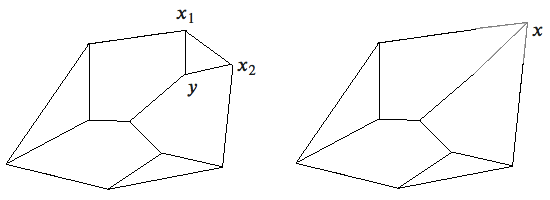
\includegraphics[width=100mm]{lifting-proof.png}
    \caption{The inductive step in the proof of Lemma~\ref{lemma:lifting}. \cite[Figure 2]{shitov2020sublinear}}
    \label{fig:lifting-proof}
  \end{figure}

  For the induction step we find a triangle with base arc $e$ like above and ``remove'' it, by continuing the arcs next to it (see Figure~\ref{fig:lifting-proof}). The continuation meets on the ``outside'' of~$e$, since $e$ has turning angle less than $\pi$.

  From the induction hypothesis we can lift this diagram with one vertex less. We cut the resulting polyhedron by the plane defined by our triangle to get our desired polyhedron.
\end{proof}

We can now focus on the main result of the first part, which allows us to build small extended formulations by combining (``gluing'') simple extensions for a surrounding polygon.

\begin{theorem}[Gluing acute extensions together, {\cite[Theorem 28]{shitov2020sublinear}}]\label{theorem:gluing}
  Let $P$ be a polygon with vertex set $V$ and $\emptyset \neq S \subseteq V$ be a subset of all vertices. Fix $\delta \geq 1$. Assume

  (i) for any $s \in S$ there are two vertices $s'$, $s''$ on two edges of $P$ adjacent to $s$,

  (ii) there are $\delta$ points $\left\{s^1, \dots, s^\delta \right\}$ in the interior of the triangle ${T_s = \conv \left\{s,s',s''\right\}}$,

  (iii) the triangles $T_s$ are disjoint for different $s$ and

  (iv) for any $i \in \{1,\dots,\delta\}$ there exists and acute diagram $D^i$ with base face $P$ such that, for any $s \in S$, the segment between $s$ and $s^i$ is a subset of the main edge of $D^i$ passing from $s$.

  $$\Rightarrow \ \xc\left( \conv\left( (V \setminus S) \cup \bigcup_{s \in S} \left\{ s',s'',s^1,\dots,s^\delta \right\}  \right) \right) \leq \abs{V} + \abs{S} + \delta$$
\end{theorem}

\begin{figure}[ht]
  \centering
  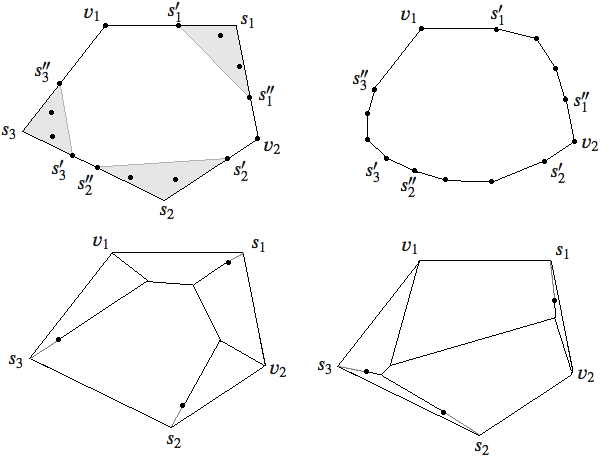
\includegraphics[width=120mm]{gluing-theorem.png}
  \caption{An application of Theorem~\ref{theorem:gluing}: Two acute diagrams confirm that the $14$-gon on the right has $\xc$ at most $10$. \cite[Figure 3]{shitov2020sublinear}}
  \label{fig:gluing-theorem}
\end{figure}

\begin{proof}
  We are going to construct a polytope $\P'$ in $\R^2 \times \R^{\delta} = \{(x,y,z^1,\dots,z^{\delta})\}$ with at most $\abs{V}+\abs{S}+\delta$ facets, which is an extended formulation of $P$.

  Assume that $a_e x + b_e y + c_e \geq 0$ is the defining inequality of an edge $e$ of $P$. Then the acute diagrams $D^i$ are lifted into three-dimensional polytopes described by $z \geq 0$ and $a_e x + b_e y + c_e \geq \varepsilon_e^i z$ with $\varepsilon_e^i > 0$ for all edges $e$ of $P$ (we assume that all diagrams are lifted into the upper half-space $z \geq 0$).

  Then we define an auxiliary polytope $\P \in \R^2 \times \R^{\delta}$ with the following $\abs{V}+\delta$ inequalities
  \begin{align*}
    a_e x + b_e y + c_e & \geq \sum_{i=1}^{\delta} \varepsilon_e^i z, \\
    z^i                 & \geq 0,
  \end{align*}
  where $e$ runs over all edges of $P$ and $i \in \{1,\dots,\delta\}$.

  We have $\dim \P = \delta + 2$, i.e.\ it has full dimension, since we can find a point $(x,y)$ in the interior of $P$ and $\varepsilon > 0$, such that $(x,y,\varepsilon,\dots,\varepsilon)$ fulfills all inequalities strictly.

  And from Observation~\ref{observation:acute-projection} we know $\pi(\P)=P$, where $\pi(x,y,z^1,\dots,z^{\delta}) = (x,y)$ is a projection.

  For any $s = (x_s, y_s) \in S$, $\sigma_s := (x_s,y_s,0,\dots,0)$ is a vertex of $\P$, since it fulfills exactly $\delta + 2$ inequalities with equality, namely $z^i \geq 0$ and the two inequalities corresponding to the edges at $s$.

  Therefore, there are $\delta + 2$ rays passing from $\sigma_s$: Two corresponding to the edges at $s$ and $\delta$ of the form
  \begin{equation}\label{eq:ray}
    (x_s + \alpha_s^i\,t,y_s + \beta_s^i\,t,0,\dots,0,t,0,\dots,0), t \geq 0,
  \end{equation}
  where there are $i-1$ zeros before~$t$ and $(\alpha_s^i, \beta_s^i)$ is pointing from $s$ to $s^i$ (and scaled such that we don't need a factor for~$t$).

  Now we define a half-space $H_s$, whose defining hyperplane is determined by the points $(x_{s'},y_{s'},0,\dots,0)$, $(x_{s''},y_{s''},0,\dots,0)$ and the $\delta$ points on \eqref{eq:ray}, which project to $s^i$ under $\pi$ (this hyperplane is well-defined, as all those points are linearly independent). The orientation of $H_s$ is set such that it does not include $\sigma_s$.

  \begin{figure}[ht]
    \centering
    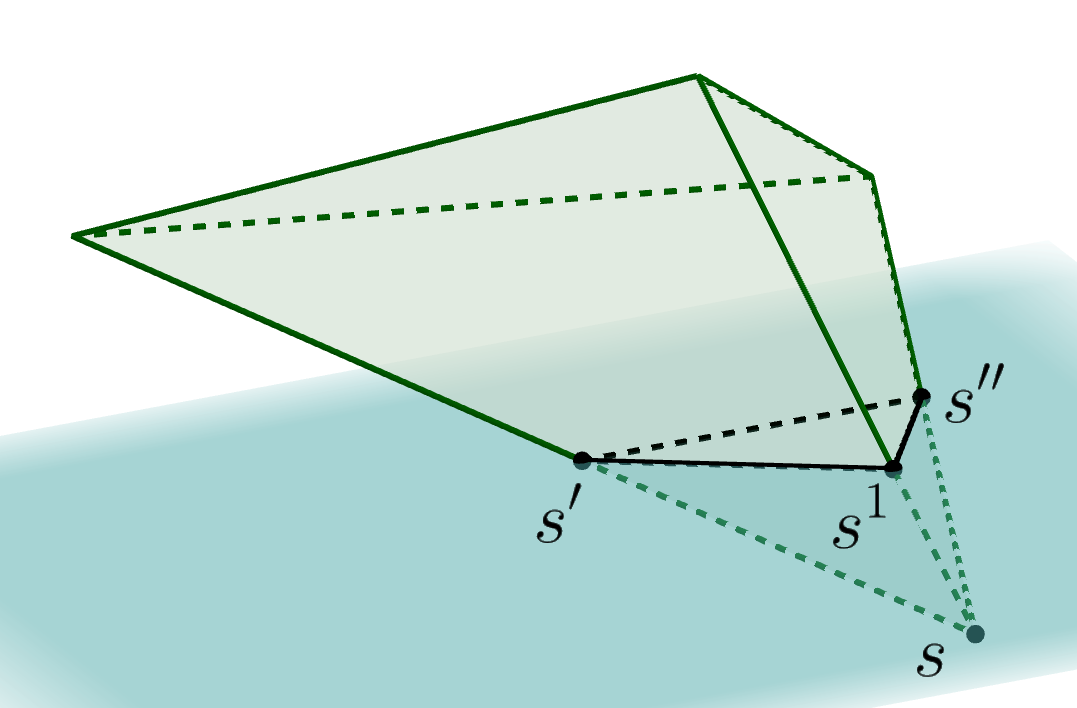
\includegraphics[width=70mm]{gluing-theorem-cut.png}
    \caption{Cutting $P$ with $H_s$ in Theorem~\ref{theorem:gluing} for $\delta = 1$.}
    \label{fig:gluing-theorem-cut}
  \end{figure}

  If we now intersect $\P$ with $H_s$, we cut the rays passing from $\sigma_s$ at the defining points of $H_s$. Since these points are all contained in an edge of $\P$ (by definition of $D^i$), these $\delta + 2$ points become vertices by this cut. The different cuts themselves don't overlap on $\P$, since the triangles $T_s$ are disjoint by definition and all $s^i$ lie in the interior of $T_s$.

  So we can define $\P' = \P \cap \bigcap_{s \in S} H_s$, which is given by $\abs{V}+\abs{S}+\delta$ inequalities, and conclude that $\pi(\P')$ is the desired polygon.
\end{proof}

\begin{remark}\label{remark:pitfall}
  There is a subtle difference between Theorem~\ref{theorem:gluing} and Corollary~\ref{corollary:acute-direction}.

  In the theorem we assume that ``the segment between $s$ and $s^i$ is a \emph{subset} of the main edge'', but in the corollary we construct a diagram for which ``the main edge from $v_i$ lies on $v_i \wedge y_i$'', implying that $y_i$ can lie outside the main edge.

  So we can't just apply Theorem~\ref{theorem:gluing} to any choice of points fulfilling (i)-(iii).
\end{remark}

To understand Theorem~\ref{theorem:gluing} better, we will now look at the limits it has in application. This observation is aside from the main argument, so feel free to skip it.

\begin{observation}[Limits of Theorem~{\ref{theorem:gluing}}]\label{observation:limits-of-gluing}
  Let $P$ be a polygon with $n$ vertices. By applying Theorem~\ref{theorem:gluing} we obtain an extended formulation for $P$ with size $\Omega(\sqrt{n})$.
\end{observation}
\begin{proof}
  We set $P := \conv\left( (V \setminus S) \cup \bigcup_{s \in S} \left\{ s',s'',s^1,\dots,s^\delta \right\} \right)$ as in Theorem~\ref{theorem:gluing}. We define $v := \abs{V}$ and $s := \abs{S}$. Throughout this proof we assume that we can apply Theorem~\ref{theorem:gluing} for our choice of $v$, $s$ and $\delta$. Then
  \begin{equation}\label{eq:limit-n}
    n \leq (v-s) + s(2+\delta) = v + s(1+\delta).
  \end{equation}

  With \eqref{eq:limit-n} we can express $\delta$ dependent on $n$, $v$ and $s$:
  \begin{equation*}
    \delta \geq \frac{n-v}{s} - 1
  \end{equation*}
  We now define $\delta := (n-v)/s$ as the minimal possible value\footnote{For simplicity, we skip the case, where $(n-v)/s - 1$ is integer. The difference would only be $-1$ in the final result.} for given $n$, $v$ and $s$, since the size of the extended formulation increases with $\delta$. This way we can define $$f_n(v,s) := v + s + \delta = v + s + \frac{n-v}{s}$$ as the size of the extended formulation for given $v$ and $s$.

  $$\frac{\partial}{\partial v} f_n(v,s) = 1 - \frac{1}{s} > 0$$ shows that $v$ should be chosen minimal for minimal extension size. So we set $v = s$ according to the assumptions of Theorem~\ref{theorem:gluing}.
  \begin{align*}
    f_n(s, s)                                & = s + s + \frac{n-s}{s}                                       \\
                                             & = 2s + \frac{n}{s} - 1                                        \\
    \frac{\partial}{\partial s} f_n(s,s)     & = 2 - \frac{n}{s^2} \Rightarrow s_{min} := \sqrt{\frac{n}{2}} \\
    \frac{\partial^2}{\partial^2 s} f_n(s,s) & = \frac{2n}{s^3} > 0
  \end{align*}

  This shows that $f_n$ has a minimum at $s_{min} = \sqrt{n/2}$ with $v_{min}=s_{min}$.

  Finally, we can find the minimal value for $f_n$:
  \begin{align*}
    f_n(s_{min}, s_{min}) = 2\sqrt{2n} - 1
  \end{align*}
\end{proof}



\subsubsection{Finding Good Subsequences}

After defining this central theorem, we have to make a way to apply it to general polygons.\footnote{See Remark~\ref{remark:pitfall}, why we can't simply use Corollary~\ref{corollary:acute-direction}.}
Therefore, we formalize the notion of ``good'' sequences with respect to Theorem~\ref{theorem:gluing}.

\begin{definition}[$t$-scattered subset]
  Let $t, n \in \N$ and $G \subset \{1,\dots,n\}$. $G$ is called $t$\emph{-scattered} if for $g, g' \in G, g \neq g'$ we have $\abs{g-g'} \geq t$.
\end{definition}

\begin{definition}[G-envelope]\label{definition:g-envelope}
  Assume $n\geq 5$ is an integer and $G\subset\{3,4,\dots,n-2\}$ is a $3$-scattered subset. If $v=(v_1,\dots,v_n)$ is a thin sequence, then the $G$\emph{-envelope} of $v$ is the sequence $v_G$ obtained from $v$ by replacing the points $v_{g-1}, v_g, v_{g+1}$ with $$o_g:=(v_{g-2}\wedge v_{g-1})\wedge (v_{g+1}\wedge v_{g+2}),$$ for all $g\in G$.
\end{definition}

\begin{figure}[ht]
  \centering
  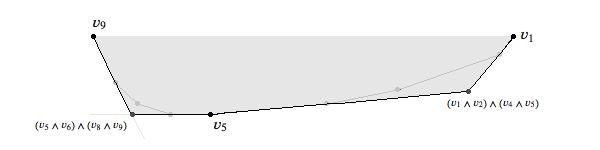
\includegraphics[width=120mm]{g-envelope.png}
  \caption{The $G$-envelope of the sequence in Figure~\ref{fig:ray-example} with $G=\{3,7\}$. \cite[Figure~6]{shitov2020sublinear}}
  \label{fig:g-envelope}
\end{figure}

\begin{definition}[G-good]
  Assume $n\geq 5$ is an integer and $G\subset\{3,4,\dots,n-2\}$ is a $3$-scattered subset. A thin sequence $v=(v_1,\dots,v_n)$ is called $G$\emph{-good} if there is an acute diagram with the base $\conv v_G$ such that, for any $g\in G$, the main edge passing from $o_g$ \emph{contains} $v_g$.
\end{definition}

Now we find another way to determine which sequences are actually \emph{G-good}. Therefore, we have to define the following:

\begin{definition}
  Let $v=(v_1,\dots,v_n)$ be a thin sequence. For indexes $i,\hat{\imath},k, \hat{\jmath}, j$ satisfying $1\leq i<\hat{\imath}<k<\hat{\jmath}<j\leq n$, we define $\rho(v,i,\hat{\imath},k, \hat{\jmath}, j)$ as the ray passing from the point $(v_i\wedge v_{\hat{\imath}})\wedge(v_{\hat{\jmath}}\wedge v_j)$ towards $v_k$.
\end{definition}

\begin{figure}[ht]
  \centering
  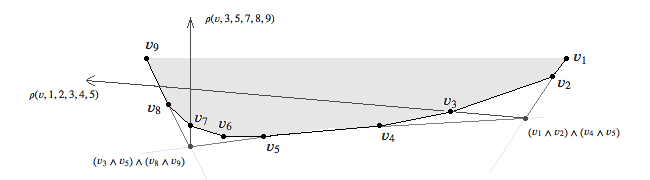
\includegraphics[width=120mm]{ray-example.png}
  \caption{Rays $\rho(v,1,2,3,4,5)$ and $\rho(v,3,5,7,8,9)$. \cite[Figure 5]{shitov2020sublinear}}
  \label{fig:ray-example}
\end{figure}

\begin{lemma}[{\cite[Lemma 42]{shitov2020sublinear}}]\label{lemma:ray-good}
  Assume $n\geq 5$ is an integer and $G\subset\{3,4,\dots,n-2\}$ is a $3$-scattered subset. Assume $v=(v_1,\dots,v_n)$ is a $\pi/2$-thin\footnote{In the source $v$ is only required to be thin, but building ``vertical'' main edges in the proof is only guaranteed to work, if both angles at $v_1$ and $v_n$ are smaller than $\pi/2$. This does not change any further proof, because this assumption is given, when this lemma gets applied.} sequence such that, for all $g\in G$, the ray $\rho(v, g-2,g-1,g,g+1,g+2)$ leaves $\conv v$ through the relative interior of the edge $\conv\{v_1, v_n\}$. Then $v$ is $G$-good.
\end{lemma}

\begin{figure}[ht]
  \centering
  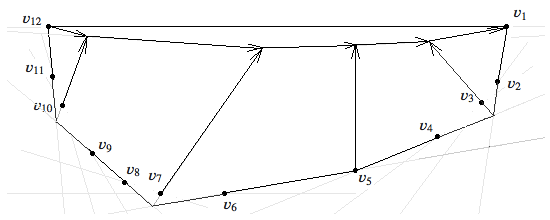
\includegraphics[width=120mm]{ray-good.png}
  \caption{An instance of Lemma~\ref{lemma:ray-good} with $n=12$ and $G=\{3,7,10\}$. \cite[Figure 7]{shitov2020sublinear}}
  \label{fig:ray-good}
\end{figure}

\begin{proof}
  To prove that $v$ is $G$-good, we build an acute diagram $\Delta$ whose base is the $G$-envelope $v_G$ of $v$ and show that the main edge passing from $$o_g := (v_{g-2} \wedge v_{g-1}) \wedge (v_{g+1} \wedge v_{g+2})$$ contains $v_g$ for each $g \in G$.

  First we build an acute diagram $\Delta$ using Corollary~\ref{corollary:acute-direction} with base $v_G$ and\\
  (1) for each $g \in G$ the main edge from $o_g$ goes towards $v_g$,\\
  (2) for each $k \notin \{1,n,g-1,g,g+1\}$ the main edge from $v_k$ is orthogonal to $v_1 \wedge v_n$,\\
  (3) the main edge from $v_n$ passes towards a point $u_0$ that lies sufficiently close to the middle of $\conv \{v_1,v_n\}$ in the interior of $\conv v$.

  Now it remains to show that the edge passing from $o_g$ actually contains $v_g$. We will prove this by contradiction: Assume there is some $j \in G$, for which $v_j$ is not contained in the edge passing from $o_j$. That is, there is an edge in $\Delta$, which has its endpoint $e$ in the interior of $\conv \{o_j, v_j\}$, thus outside of $\conv v$.

  \textit{Case 1.} There is a path of inner arcs in $\Delta$ from $v_n$ to $v_1$, including $e$.\\
  This is impossible, because the main edge passing from $v_n$ leaves towards $u_0$, thus not leaving $\conv v$. This follows from property (v) in Lemma~\ref{lemma:diagram-properties}, because an inner arc of $\Delta$ on the path from $v_n$ to $v_1$ separating the face containing $v_1 \wedge v_n$ and the face containing $v_i \wedge v_{i+1}$ continues to arc ``towards'' $v_1$ for decreasing $i$, because $v$ itself is convex.\footnote{The line through this arc has to be concurrent with $(v_1 \wedge v_n) \wedge (v_i \wedge v_{i+1})$, which is a point on $v_1 \wedge v_n$ outside $\conv \{v_1,v_n\}$, because of the convexity of $v$. This arc can't be moving away from $v_n$ steeper than $v_n \wedge u_0$.}

  \textit{Case 2.} There is \emph{no} path of inner arcs in $\Delta$ from $v_n$ to $v_1$, including $e$.\\
  All main edges of $\Delta$ go towards the interior of $\conv \{v_1, v_n\}$ (except the two at $v_1$ and $v_n$). And any path from a base vertex of $\Delta$ to $v_1$ that includes $e$ has to leave $\conv v$. This path can only leave through the interior of $\conv\{v_1,v_n\}$ because of (v) in Lemma~\ref{lemma:diagram-properties} and the convexity of $v$.\footnote{For any intersection point, there is a leftmost incoming arc $f$ and a rightmost incoming arc $g$, which are concurrent with the base edges $f_l$, $f_r$ respectively $g_l$, $g_r$. So the outgoing arc $h$ is concurrent with $f_l$ and $g_r$, which fixes it inside the cone spanned by continuing $f$ and $g$.}
  So it has to intersect the path from $v_n$ to $v_1$ before leaving $\conv v$. This contradicts the assumption of this case.

  So it is proved that the edge passing from $o_g$ contains $v_g$ for all $g \in G$.
\end{proof}

We now need to define one more property of a sequence, by which we will split our upcoming considerations.

\begin{definition}[Slanted sequence]
  Let $v=(v_1,\ldots,v_t)$ be a thin clockwise sequence, ${\beta\in(0,\pi/2)}$, $\delta\geq 0$. We say that $v$ is \emph{clockwise-slanted} to an angle $\beta$ with \emph{tolerance} $\delta$, if, for all $i,\hat{\imath},\hat{\jmath}, j$ satisfying $1\leq i<\hat{\imath}<\hat{\jmath}<j\leq t$, the ray ${\rho}(v,i,\hat{\imath},k,\hat{\jmath}, j)$ satisfies $$\angle\left(\overrightarrow{v_{\hat{\jmath}}\wedge v_j},\,\,\rho(v,i,\hat{\imath},k,\hat{\jmath}, j)\right)<\beta$$ for all $k$ satisfying $\hat{\imath}<k<\hat{\jmath}$ except for at most $\delta$ such values of $k$.

  A \emph{counterclockwise-slanted} sequence is a counterclockwise sequence, if the above definition holds with ``clockwise'' replaced with ``counterclockwise''.
\end{definition}

\begin{figure}[ht]
  \centering
  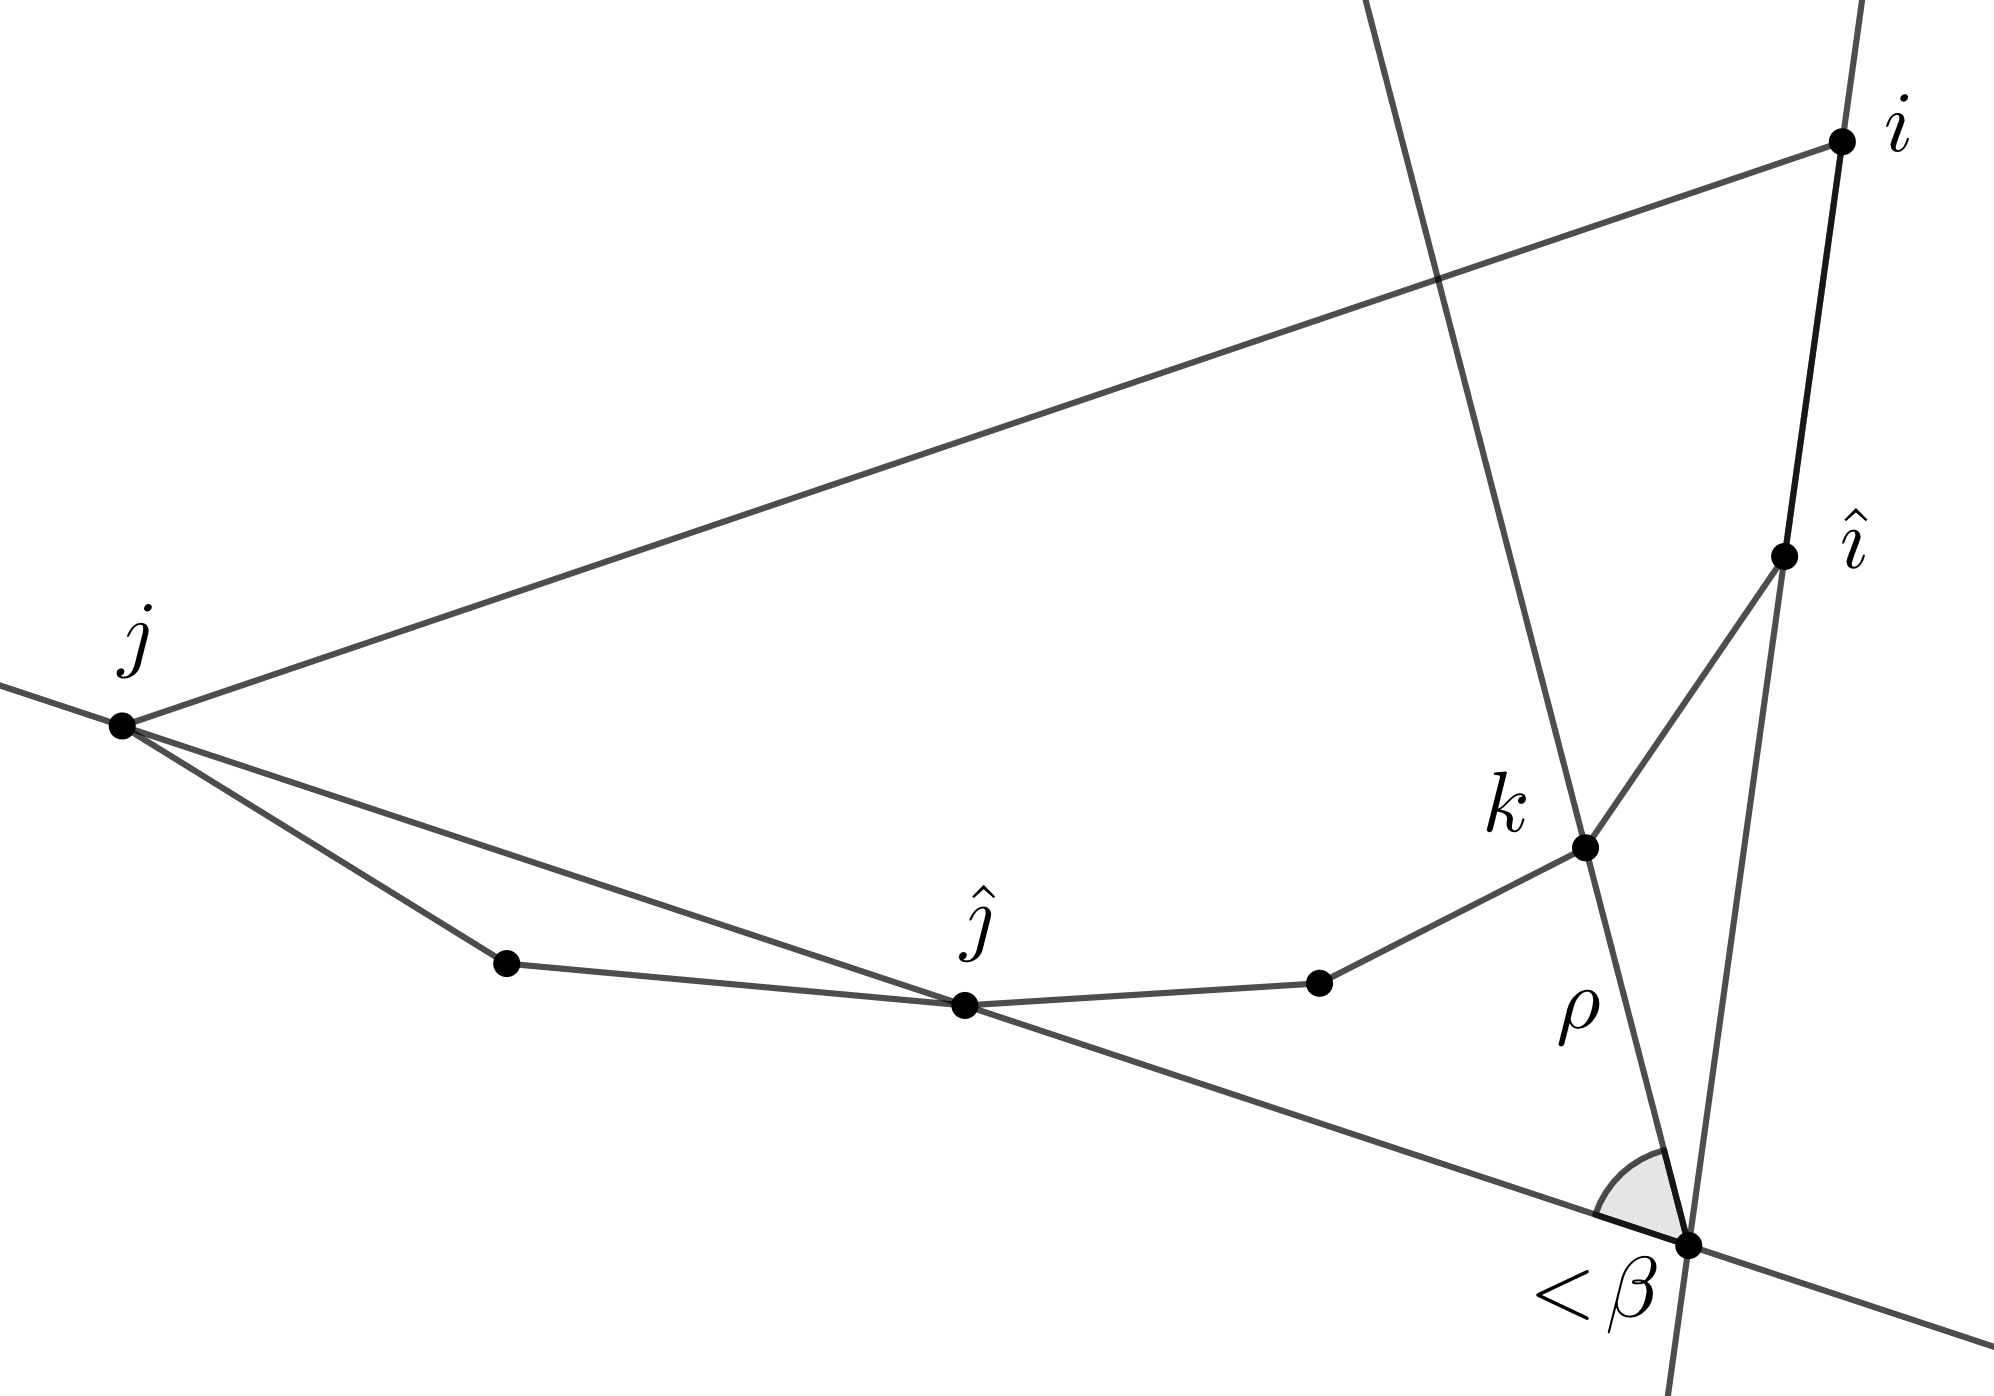
\includegraphics[width=100mm]{slanted.png}
  \caption{Points and angles used in the definition of slanted sequences.}
  \label{fig:slanted}
\end{figure}

Note that we couldn't come up with an intuitive understanding of slanted sequences. If $k$ goes around in clockwise direction, the measured angle decreases, so vertices failing the condition are consecutive starting after $\hat{\imath}$. And if one fixes $k$, $\hat{\jmath}$ and $j$, moving $i$ or $\hat{\imath}$ in clockwise direction will increase the measured angle. But the same can't be done for $j$ and $\hat{\jmath}$. So this definition serves its purpose in the proofs, but doesn't provide more insight beyond that.

Now we split the search for a good subsequence into two cases:
\begin{enumerate}
  \item The original sequence has a large enough slanted subsequence.
  \item The original sequence does not have such a subsequence.
\end{enumerate}

We can show that for each case there is a large enough subsequence, for which Theorem~\ref{theorem:gluing} can be applied well. This is done in the following lemmata, for which we will skip the technical proofs, since they provide little insight.

\begin{lemma}[{\cite[Lemma 49]{shitov2020sublinear}}]\label{lemma:unslanted-subseqence}
  Let $\delta, \tau, m$ be positive integers and $n=8\tau m$. Let $\alpha,\beta$ be positive reals with $\pi/2>\beta\geq 2\alpha$. Assume $v=(v_1,\dots,v_n)$ is an $\alpha$-thin sequence such that any subsequence with $m$ points is neither clockwise-slanted nor counterclockwise-slanted relative to the angle $\beta$ and tolerance $2\delta$. Then $v$ has a subsequence with $(6+\delta)\tau$ points with extension complexity not exceeding $6\tau+\delta+1$.
\end{lemma}

\begin{lemma}[{\cite[Theorem 57]{shitov2020sublinear}}]\label{lemma:slanted-subsequence}
  Let $\delta>1$ be an integer and $n=8\delta^2$. Let $v=(v_0,\ldots,v_n)$ be a $\pi/6$-thin sequence that is clockwise-slanted to the angle $\pi/3$ with tolerance~$2\delta$. Then $v$ has a subsequence of size at least $0.25\delta^2$ and extension complexity at most $3\delta$.
\end{lemma}

Now we have all building blocks to tackle proving Theorem~\ref{theorem:subsequence}, which states that a $\pi/6$-thin sequence $v$ with $n = 1024\tau^3 + 8\tau$ vertices it contains a subsequence $u$ with $\abs{u} \geq 4\tau^2$ and $\xc(u) \leq 12\tau$.\\
In light of \ref{observation:limits-of-gluing} this subsequence makes optimal use of Theorem~\ref{theorem:gluing} in an asymptotical way.

\begin{proof}[Proof outline of Theorem~\ref{theorem:subsequence}]
  We try to apply Lemma~\ref{lemma:unslanted-subseqence} with $\beta = \pi/3$, $\delta = 4\tau$ and $m = 8\delta^2 + 1$.

  If it is applicable, $v$ contains a subsequence with the desired properties.

  If it isn't applicable, $v$ has a subsequence $u$, which is slanted to the angle $\pi/3$ with tolerance $2\delta$. By Lemma~\ref{lemma:slanted-subsequence} $u$ contains a subsequence with the desired properties.
\end{proof}



\subsubsection{Conclusion}

Now we have proved that $\xc(P) \in O(n^{2/3})$ for any $n$-gon $P$, which leaves us wondering if this bound can be improved further, since the lower bound is $\xc(P) \in \Omega(n^{1/2})$ for some $n$-gon $P$.

Looking back at the key ideas, we see that Theorem~\ref{theorem:gluing} was used optimally for each subsequence (see Observation~\ref{observation:limits-of-gluing}). If we wanted to improve the bound using this theorem, we would have to find larger subsequence, for which we can apply it.

Theorem~\ref{theorem:subsequence} shows that we can find a subsequence with $m \in \Omega(n^{2/3})$ vertices with extension complexity in $O(m^{1/2})$, i.e.\ for which Theorem~\ref{theorem:gluing} is used asymptotically optimal. If we could find a subsequence with $m \in \Theta(n)$ vertices, for which we can apply Theorem~\ref{theorem:gluing} (asymptotically) optimal, we would achieve a final result of $\xc(P) \in O(n^{1/2})$ for any $n$-gon $P$, which would close the gap between lower and upper bound.


